\documentclass{article}
\usepackage[utf8]{vietnam}
\usepackage{amsmath}
\usepackage{tikz}
\usetikzlibrary{arrows.meta,automata,positioning,shadows}

\title{The first document }
\author{Your Name}
\date{\today}

\begin{document}
	
	\maketitle
	\section{Introduction}
	Hello LaTeX!
	\subsection{Introduction}
	Math equation: $E = mc^2$.
	Second equation:
	$$ \int_{a}^{b} f(x) \,dx = F(b) - F(a) $$
	My name is Đỗ Thành Trung.
	\begin{abstract}
		\textbf{This is the abstract of the document.}
		\textbf{I am working as a System Engineer.}
		The following formula is written in LaTeX:
	\end{abstract}
	$$ \begin{aligned}
& {\left[\begin{array}{c}
\hat{\operatorname{Re}}\left(\omega_1\right) \\
\ldots \\
\hat{\operatorname{Re}}\left(\omega_n\right) \\
\hat{\operatorname{Im}}\left(\omega_1\right) \\
\ldots \\
\hat{\operatorname{Im}}\left(\omega_n\right)
\end{array}\right]=\left[\begin{array}{l}
\varepsilon_R\left(\omega_1\right) \\
\ldots \\
\varepsilon_R\left(\omega_N\right) \\
\varepsilon_I\left(\omega_1\right) \\
\ldots \\
\varepsilon_I\left(\omega_N\right)
\end{array}\right]+} \\
& {\left[\begin{array}{llllllllll}
1 & 0 & -\omega_1^2 & 0 & \omega_1^4 & \ldots & \hat{\operatorname{Im}}\left(\omega_1\right) \omega_1 & \hat{\operatorname{Re}}\left(\omega_1\right) \omega_1^2 & -\hat{\operatorname{Im}}\left(\omega_1\right) \omega_1^3 & \ldots \\
\ldots & \ldots & \ldots & \ldots & \ldots & \ldots & \ldots & \ldots & \ldots & \ldots \\
1 & 0 & -\omega_N^2 & 0 & \omega_N^4 & \ldots & \hat{\operatorname{Im}}\left(\omega_N\right) \omega_N & \hat{\operatorname{Re}}\left(\omega_N\right) \omega_N^2 & -\hat{\operatorname{Im}}\left(\omega_N\right) \omega_N^3 & \ldots \\
0 & \omega_1 & 0 & -\omega_1^3 & 0 & \ldots & -\hat{\operatorname{Re}}\left(\omega_1\right) \omega_1 & \hat{\operatorname{Im}}\left(\omega_1\right) \omega_1^2 & \hat{\operatorname{Re}}\left(\omega_1\right) \omega_1^3 & \ldots \\
\ldots & \ldots & \ldots & \ldots & \ldots & \ldots & \ldots & \ldots & \ldots & \ldots \\
0 & \omega_N & 0 & -\omega_N^3 & 0 & \ldots & -\hat{\operatorname{Re}}\left(\omega_N\right) \omega_N & \hat{\operatorname{Im}}\left(\omega_N\right) \omega_N^2 & \hat{\operatorname{Re}}\left(\omega_N\right) \omega_N^3 & \ldots
\end{array}\right]\left[\begin{array}{l}
b_0 \\
\ldots \\
b_m \\
a_1 \\
\ldots \\
a_n
\end{array}\right]}
\end{aligned} $$
$$
\begin{aligned}
& \frac{-b \pm \sqrt{b^2-4 a c}}{2 a} \frac{-b \pm \sqrt{b^2-4 a c}}{2 a} \frac{-b \pm \sqrt{b^2-4 a c}}{2 a} \\
& \frac{n!}{r!(n-r)!} \frac{n!}{r!(n-r)!} \frac{n!}{r!(n-r)!} \frac{n!}{r!(n-r)!} \lim _{x \rightarrow \infty}
\end{aligned}
$$

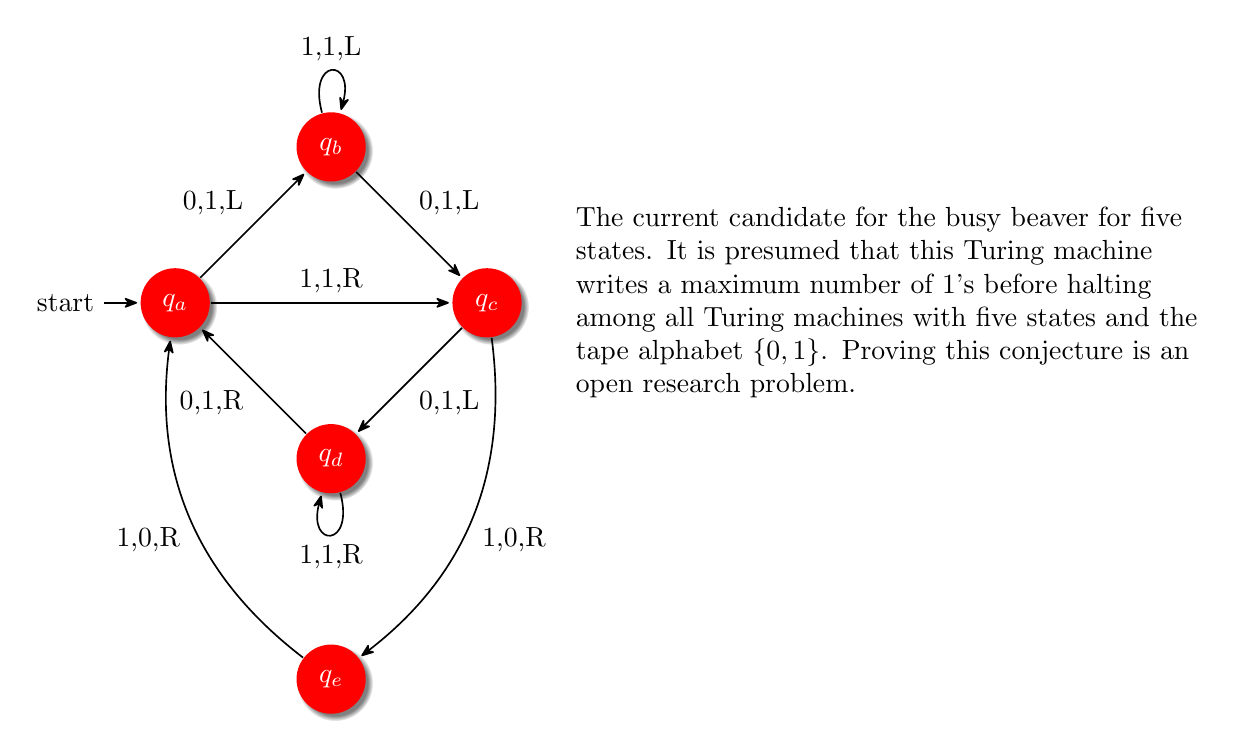
\begin{tikzpicture}[->,>={Stealth[round]},shorten >=1pt,auto,node distance=2.8cm,on grid,semithick,
                    every state/.style={fill=red,draw=none,circular drop shadow,text=white}]

  \node[initial,state] (A)                    {$q_a$};
  \node[state]         (B) [above right=of A] {$q_b$};
  \node[state]         (D) [below right=of A] {$q_d$};
  \node[state]         (C) [below right=of B] {$q_c$};
  \node[state]         (E) [below=of D]       {$q_e$};

  \path (A) edge              node {0,1,L} (B)
            edge              node {1,1,R} (C)
        (B) edge [loop above] node {1,1,L} (B)
            edge              node {0,1,L} (C)
        (C) edge              node {0,1,L} (D)
            edge [bend left]  node {1,0,R} (E)
        (D) edge [loop below] node {1,1,R} (D)
            edge              node {0,1,R} (A)
        (E) edge [bend left]  node {1,0,R} (A);

   \node [right=1cm,text width=8cm] at (C)
   {
     The current candidate for the busy beaver for five states. It is
     presumed that this Turing machine writes a maximum number of
     $1$'s before halting among all Turing machines with five states
     and the tape alphabet $\{0, 1\}$. Proving this conjecture is an
     open research problem.
   };
\end{tikzpicture}

\end{document}